\label{sec:justificacion_y_objetivos}

\subsection{Acerca del proyecto}

El presente Trabajo Fin de Grado, parte de un programa ya preexistente que se usa y estudia en la asignatura Tecnologías Multimedia el cual se llama \textit{Intercom}. El sistema \textit{Intercom} es una solución de comunicación bidireccional, al principio solo de audio pero este trabajo, trata y logra solucionar el mismo problema implementando además, la transmisión simultánea de vídeo. Dicho programa permite la transmisión de audio y vídeo en tiempo real simultaneamente. Su diseño se enfoca en la eficiencia y calidad de la señal de audio asi como, la eficiencia y distintas posibles configuraciones de vídeo pudiendo cambiar tanto la resolución del mismo y su \textit{FPS} (Cuadros por segundo, Frame Rates per Second por sus siglas en inglés). Este sistema está preparado para ejecutarse en entornos con limitaciones de ancho de banda y en practicamente cualquier dispositivo por poco potente que sea debido a su alta eficiencia y poca complejidad computacional.
\vspace{\baselineskip}

Dicho programa, \textit{Intercom}, que se encuentra en el repositorio de la asigntuara\footnote{https://github.com/Tecnologias-multimedia/InterCom}, utiliza técnicas avanzadas de procesamiento de señales así como implemnta diversos algoritmos de compresión de datos y optimización de la transmisión de flujos multimedia a través de los disversos módulos que contiene el mismo. 

\vspace{\baselineskip}
Todo el codigo, tanto preexiste como implemetado en este trabajo, es en el leguaje de programación Python. Ademas, para la realizacion de esta memoria, ha sido redactada y compuesta en su totalidad en lenguaje LaTex, un sistema de preparación de documentos que permite la creación de documentos de alta calidad tipográfica y es ampliamente utilizado en el ámbito académico y científico. La elección de LaTeX para la redacción de esta memoria no solo garantiza una presentación profesional, sino que también facilita la inclusión de tablas, gráficos y referencias bibliográficas de manera eficiente, personalizada y organizada.

\vspace{\baselineskip}
\begin{center}
	
\includegraphics[width = 0.25\textwidth]{images/LaTeX_logo.png}
	\captionof{figure}{Logo de LaTeX}
	\label{fig:latex}
\end{center}
\vspace{\baselineskip}

\subsection{Justificación y objetivos del proyecto}
La justificación de este proyecto está claramente fundamentada en diversos factores que son altamente relevantes en los tiempos actuales, sobre todo en las áreas académicas, tecnológicas y sociales. Evidentemente, en el mundo tan interconectado en el que vivimos, la comunicación multimedia ha adquirido una importancia crucial en múltiples ámbitos, desde la educación hasta el ámbito profesional y personal. La necesidad de herramientas eficientes y efectivas para la comunicación audiovisual es cada vez más evidente, especialmente en un contexto donde la interacción a distancia se ha vuelto la orden del día.\cite{GSMA}
\vspace{\baselineskip}

El objetivo principal es facilitar una comunicación clara y fluida, que ya existía en la versión antigua de \textit{InterCom} con el audio, mejorándola con el añadido además, como ya se ha comentado, de la transmisión simultánea de audio y vídeo, permitiendo distintas configuraciones de parámetros de vídeo. Principalmente, lo que se busca con este proyecto es la investigación y desarrollo de la herramienta \textit{Intercom} en un enfoque académico, en el cual se expanda el funcionamiento actual del mismo para descubrir nuevas maneras de desarrollar y profundizar en la herramientas de intercomunicación, como se ha hecho en el caso del vídeo en este proyecto.

\vspace{\baselineskip}
Evidentemente, se desea lograr este objetivo intentando minimizar la latencia y el uso de recursos de red que es esencial en estos programas de intercomunicación~\cite{cisco}, aunque el programa esta preparado para más situaciones diversas.

\vspace{\baselineskip}

Entre los objetivos del proyecto estan:

\begin{itemize}
	\item Desarrollar los sistemas necesarios para la captura, transmisión, recepción y visualización del vídeo en tiempo real, fundamentales para la realización de este proyecto.
	\item Garantizar la compatibilidad con el subsistema de audio preexistente y los módulos derivados.
	\item Desarrollo de diversos módulos adicionales para mejorar/adaptar el programa teniendo en cuenta distintas situaciones posibles de ejecución por parte del usuario. Entre ellas, la ejecución del programa con resoluciones distintas a las permitidas por el dispositivo de la cámara asi como, ajustar los Cuadros por Segundo (\textit{FPS}) deseados por el usuario haciendo que sean compatibles con dicha resolución.
\end{itemize}
\vspace{\baselineskip}


\subsection{Estructura de InterCom}

A continuación, para mayor contexto y comprensión del proyecto, se presenta la estructura jerarquizada de \textit{InterCom} que ilustra la organización de los módulos y componentes del sistema. Esta representación visual proporciona una visión clara de cómo se interrelacionan los diferentes elementos del programa.
\vspace{\baselineskip}

Antes de la realización de este proyecto, el sistema \textit{InterCom} contaba con una estructura jerarquizada que se puede observar en la figura \ref{fig:jeraquia}, que se mostrará a continuación, excluyendo los módulos de \textit{Minimal\_Video} y los adicionales implementados tambien en este trabajo que son \textit{Minimal\_Video\_FPS} y \textit{Minimal\_Video\_Resolution}. 

\vspace{\baselineskip}
Por lo tanto, al implementar los nuevos módulos, la estructura quedaría de la sigueinte manera:

\begin{center}
	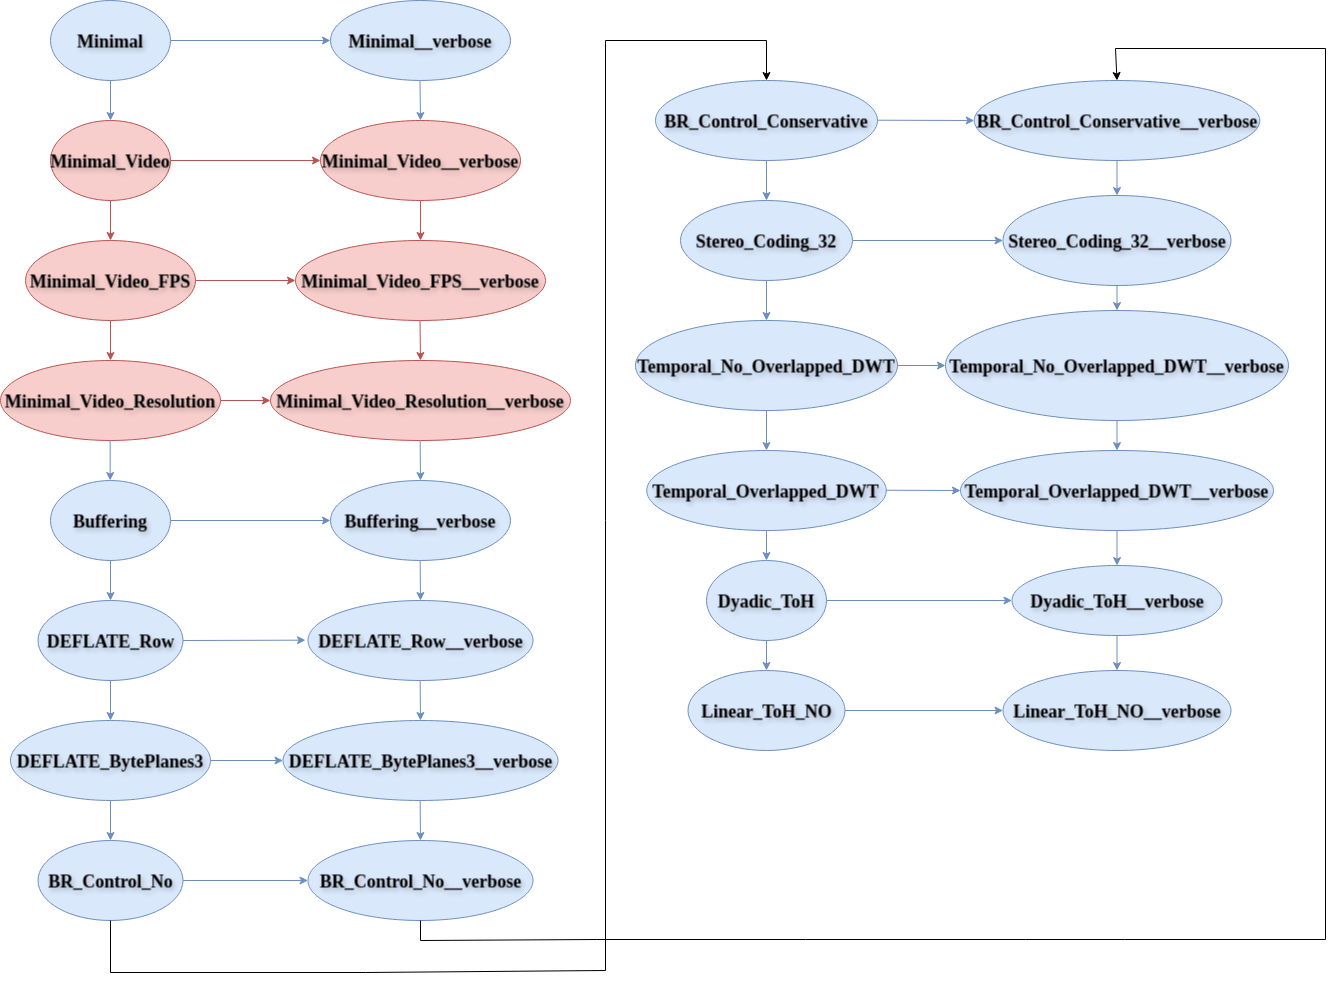
\includegraphics[width = 1.1\textwidth]{images/jerarquia_modulos.png}
	\captionof{figure}{Estructura jeraquizada de InterCom}
	\label{fig:jeraquia}
\end{center}

\vspace{\baselineskip}
Como se puede observar en la figura, el sistema se compone de varios módulos, cada uno de los cuales desempeña un papel específico en la funcionalidad general del programa. El programa base o padre es \textit{Minimal} cuya función es la transmisión sin compresión, sin cuantificación, sin transformación, simplemente una transmisión bidireccional (\textit{full-duplex}) de trozos (\textit{chunks}) sin procesar y que sean reproducibles. De este módulo, parten todos los demás módulos que componen \textit{InterCom}, incluyedo los nuevos implementados. 
\vspace{\baselineskip}

Por mencionar algunos de los módulos que se pueden observar en la figura \ref{fig:jeraquia} y su funcionamiento, por ejemplo, el módulo \textit{Buffering.py} implementa una estructura de búfer de acceso aleatorio para ocultar el jitter\footnote{El jitter simplemente es la fluctuación a la variabilidad temporal durante el envío de señales digitales, una ligera desviación de la exactitud de la señal de reloj. El jitter suele considerarse como una señal de ruido no deseada.}. Otro módulo que puede ser digno de mención es \textit{DEFLATE\_raw.py}, que implementa el algoritmo de compresión DEFLATE\footnote{El algoritmo DEFLATE se usa para la compresión de datos sin pérdidas que usa una combinación del algoritmo LZ77 y la codificación Huffman.} para comprimir cada trozo (chunk).

\vspace{\baselineskip}
En nuestro caso, nos centraremos en el módulo \textit{Minimal\_Video} y su version \textit{verbose}\footnote{La versión verbose simplemente muestra al ejecutar, estadísticas y datos adicionales a la versión normal}, que son los que estan resaltados en la figura, así como, los módulos \textit{Minimal\_Video\_FPS} y \textit{Minimal\_Video\_Resolution} y sus versiones \textit{verbose} correspondiente, que son los que se han implementado y desarrollado en este trabajo.

\vspace{\baselineskip}
Como hemos comentado, el módulo \textit{Minimal\_Video} es el encargado de la transmisión de vídeo y audio en tiempo real. Este módulo se basa en el módulo \textit{Minimal} y añade la funcionalidad de captura, transmisión y recepción de vídeo, permitiendo una comunicación multimedia más completa. La versión \textit{verbose} proporciona información adicional sobre el rendimiento del sistema durante la ejecución. Este será nuestro módulo base para los otros dos módulos adicionalmente implementados y desarrollados en este trabajo \textit{Minimal\_Video\_FPS} y \textit{Minimal\_Video\_Resolution}. En la siguiente tabla \ref{tab:modulos} se muestra una comparativa resumida de que hace cada módulo implementado asi como de quien hereda, información sobre su versión \textit{verbose} y posibles casos de uso.

\begin{center}
\captionof{table}{Comparativa de módulos implementados}
\label{tab:modulos}
\begin{tabular}{|p{2.6cm}|p{4cm}|p{4cm}|p{5cm}|}
    \cline{2-4} % Solo dibuja línea horizontal en columnas 2-4
    \multicolumn{1}{c|}{} & % Primera celda sin línea izquierda ni texto
    \textbf{Minimal\_Video} & 
    \textbf{Minimal\_Video\_FPS} & 
    \textbf{Minimal\_Video\_Resolution} \\
    \hline
    \textbf{Funcionalidad principal} & 
    Transmisión de vídeo y audio en tiempo real & 
    Ajuste de FPS según la resolución & 
    Configuración y reescalado a una resolución compatible \\
    \hline
    \textbf{Hereda de} & 
    Minimal & 
    Minimal\_Video & 
    Minimal\_Video\_FPS \\
    \hline
    \textbf{Versión verbose} & 
    Muestra estadísticas de rendimiento en tiempo real & 
    Incluye información sobre el ajuste de FPS realizado & 
    Muestra datos sobre el reescalado, la resolución y compatibilidad \\
    \hline

    \textbf{Caso de uso} & 
    Comunicación multimedia básica & 
    Cuando se requiere control específico de Cuadros por Segundo (\textit{FPS}) & 
    Cuando la resolución solicitada por el usuario no es compatible \\
    \hline
\end{tabular}
\end{center}
\vspace{\baselineskip}

Con esto acaba el capítulo de \textit{Introducción}. En el siguiente capítulo, se presentará la metodología utilizada para el desarrollo del proyecto, incluyendo los pasos seguidos y las herramientas empleadas así como, la explicación completa del código desarrolado. Se detallarán los aspectos técnicos y las decisiones tomadas durante el proceso de implementación de los módulos adicionales implementados en \textit{InterCom}.